\section{DSM Performance Assessment} % (fold)
\label{sec:index}
We identify four requirements for performance assessment of DSM:
\begin{itemize}
	\item[R1] Provide a \emph{quality} measure normalized to the contractual requirements (bounds) of a service. By normalizing the quality measure to the bounds, the \emph{QoS} value for both ancillary services and asset-management services will have comparable dimensions.
	\item[R2] The measure should be normalized with respect to time.
	\item[R3] Provide a \emph{reliability} measure in relation to service non-delivery.
	\item[R4] Each service must have a separate, individually verifiable, measure. For example, to evaluate service delivery w.r.t. ancillary-service delivery, the asset-management quality is irrelevant.
\end{itemize}

To satisfy these requirements, we propose a performance index quantifying the quality of ancillary services and asset-management services, and a non-delivery counter (NDC) which increases every time the QoS is out of bounds. Normalization is based on a scaling factor modeled after the contractual limits of the respective service. The limits are defined via a contract with the entity requesting the service. Thus, the performance index is specifically designed to evaluate how well the service provision conforms to the contractual boundaries.
	%The formulation of a performance index transforms the service requirements of the Aggregator into a single computable quality measure. %The index presented here is defined for post-simulation analysis, and represents the performance of the control algorithm over the whole time horizon. 
	\subsection{Definition of the performance index}
	In previous sections we have defined the concept of QoS as a deviation, $e(t)$, from a contracted behavior. Since there is a contractual limit on the allowed deviation, the error is normed to be a percentage of this limit such that:
	\begin{equation}
		QoS_{s}(t)=|e(t)|C_{s}(t); \quad  QoS_{s}(t)\in [0,1]
	\end{equation}
	where \emph{s} is either \emph{AS} for ancillary service or \emph{AMS} for asset-management service, and $C_s(t)$ is the corresponding normalization factor derived from the service model. When $QoS_{AS}(t) \geq 1$, the measure for reliability NDC is increased. %For the ancillary services this is simply expressed as $QoS_{AS}(t) = e(t)_{AS}$ while the expression for the asset management service is $QoS_{AM}(t) =\sum_{k=1}^M e(t)_{AM}$.

	Using the square root of the Integral Square Error index (i.e. the 2-norm, as defined in e.g. \cite{Skogestad}), the following performance criterion is defined for service delivery seen from the Aggregator perspective:
	\begin{equation}
		%\text{J}=\sqrt{\int_{0}^{N}\left( \sum_{k=1}^M |e(t)_{AM,k}C_{AM}|^{2}+|e(t)_{AS}C_{AS}|^{2}\right)dt} 
		{J}(N)=\sqrt{\int_{0}^{N}\left( \sum_{k=1}^M {QoS}_{AMS,k}(t)^{2}+{QoS}_{AS}(t)^{2}\right)dt} 
	\end{equation}
where ${QoS}_{AM,k}(t)$ and ${QoS}_{AS}(t)$ are the time-dependent measures of service quality for the asset-management service and the ancillary service, respectively. The units controlled by the Aggregator are denoted by the index \emph{k}, the unit portfolio is of size \emph{M}, and \emph{N} is the time horizon over which the services are provided. %Finally, $Q_D$ and $Q_U$ are scaling factors that convert the errors into percentages so that $e(t)_D$ and $e(t)_U$ are comparable. 
While the index~\eqref{eq:astrom} benchmarks the actual performance criterion against a theoretical minimum, we benchmark it against the worst case scenario $J_{max}$, such that the performance index is given by:
	\begin{equation} 
		\eta = \frac{J_{act}(N)}{J_{max}(N)}\label{eq:eta}
	\end{equation}
	where $\eta \in [0,1)$ for a valid service delivery and for which values close to zero represent good performance of service delivery. If $\eta \geq 1$ the Aggregator does not perform according to its service contract.
		
		Normalization with respect to time is achieved when benchmarking against $J_{max}(N)$, since $J_{max}(N)$ is estimated by integrating over the service delivery period. Contrary to index \eqref{eq:astrom}, which gives an intuition of how close performance is to the optimum, index \eqref{eq:eta} gives an intuition of how far performance is from the worst case scenario. The index is designed this way because the theoretical optimum of service delivery is $J_{opt}=0$, i.e. no error in service delivery.
	%It must be noted that the performance criterion only measures the permissible error defined in the contract of the service (the service quality), and service non-delivery (the service reliability) is measured separately. Therefore, whenever the algorithm performs outside the established limits, then $J(t)_{act}=J(t)_{max}$ and a non-delivery counter is increased.
	\subsection{Calculating the index}\label{sub:modelcalc}
	Having defined what the performance index measures, we will proceed with establishing how to obtain the required values to estimate the index. Calculating the performance index requires the following steps:
	% the maximum permissible error ($J(t)_{max}$) of the service requires two steps:
		\begin{enumerate}
		\item Identify and model the service requirements and errors in service provision, giving the scaling factor $C(t)_s$.
			\item Estimate $J_{act}(N)$.
			\item Calculate \emph{J(N)} for operation on the requirement boundaries ($J_{max}(N)$).
			\item Calculate $\eta$ by benchmarking $J_{act}(N)$ with $J_{max}(N)$.
		\end{enumerate}	
		
	For the first step, the service requirements must be defined and translated into measurable errors. For some services, the error can be stated as a tracking error, e.g. $e=y_{ref}-y_{meas}$. In other cases, service requirements are defined by operation within bands, which may lead to an error defined as:
	\begin{equation}
	e(x)= \left\{ \begin{array}{l l}
	x_{min} - x & \quad \text{ if } x \leq x_{min}\\
	0 & \quad \text{ if } x_{min} \leq x \leq x_{max}\\
	x - x_{max} & \quad \text{ if } x \geq x_{max}
	\end{array} \right.
	\end{equation}
	This step is a service-specific problem and is non trivial.

	The second step requires computing $J_{act}(N)$ using measurement data from the unit portfolio. This can be a challenge for evaluation in field deployment. In this paper it is assumed that the measurement data is available, either through a DSO or a third-party metering company.	
	
		%The actual performance of the aggregation algorithm can be found through two different methods:
%\begin{itemize}
	%\item On-line monitoring -- This method brings the added benefit of being able to use the index for performance monitoring and diagnosis at runtime, but the downside of being communication intensive.  
	%\item Post-delivery analysis -- This method is less communication intensive, but does not permit to take remedial actions at run time if a aggregation controller is not working as expected.
%\end{itemize}
%	Usually services have some acceptable error (see Sec.~\ref{sub:ancillary}) which can be interpreted as the hard boundaries for the service delivery.
	The third step requires the calculation of \emph{J(N)} along the contractual boundaries for service delivery, in this way, the maximum allowed error is found for the service. The boundaries are based on the service models presented in the first step. By adding the maximum permissible error for all services, $J_{max}(N)$ is obtained. 
	%Normalizing the performance measure with the $J_{max}$ gives an intuitive value of the performance of the control algorithm.
	The following subsection present an example of how to determine $J_{max}(N)$.

	\subsection{An example: DSO Service PowerMax}\label{sub:example}
	For demonstration purposes, in this section $J_{max}(N)$ for the PowerMax service is calculated. 
	Typically, the service will be contracted several months ahead of the actual delivery. The activation schedule (On and Off triggers), the maximum power cap ($P_M$), the maximum duration of the service per activation ($T_M$), and the quality of service (\emph{QoS}) are defined when contracting the service. The contract is valid for a period of several months, where the Aggregator is obliged to follow the established schedule.

	The limits specified for the QoS\cite{FLECH} of the PowerMax service are presented here: 
	\begin{itemize}
		\item Deviation from On trigger: $\pm$ 15 min. per day
		\item Deviation in size of service (dependent on $P_M$): Max. $\pm 5\% P_M$  
		\item Acceptable no. of unsatisfactory activations(non-delivery): $\text{NDC} = 4$
	\end{itemize}

A graphical representation of these service requirements is depicted in Fig.~\ref{fig:servicereq}. It is clear that the maximum acceptable error in service delivery is the shaded area. Note that the limit for non-delivery of service during the first 15 minutes of activation is dotted due to the fact that non-delivery is not counted during this period. The specifications for counting unsatisfactory activations are not clarified in \cite{FLECH}, so it is assumed that breaking the QoS limits on one sampling period counts as one non-delivery. In the case where the service is not respected in three consecutive (or non-consecutive) sampling periods, $\text{NDC}=3$.

For example, in the case where  $P_M = 5\,kW$, $T_M=4\, h$ and the power is measured once an hour, $J_{max}(N) = 2$, as it represents the square root of the square of the maximum (when $J_{act}(N)=1$) permissible error over 4 hours.
\begin{figure}[t]  % Find out how to send it to next column.
	\centering
	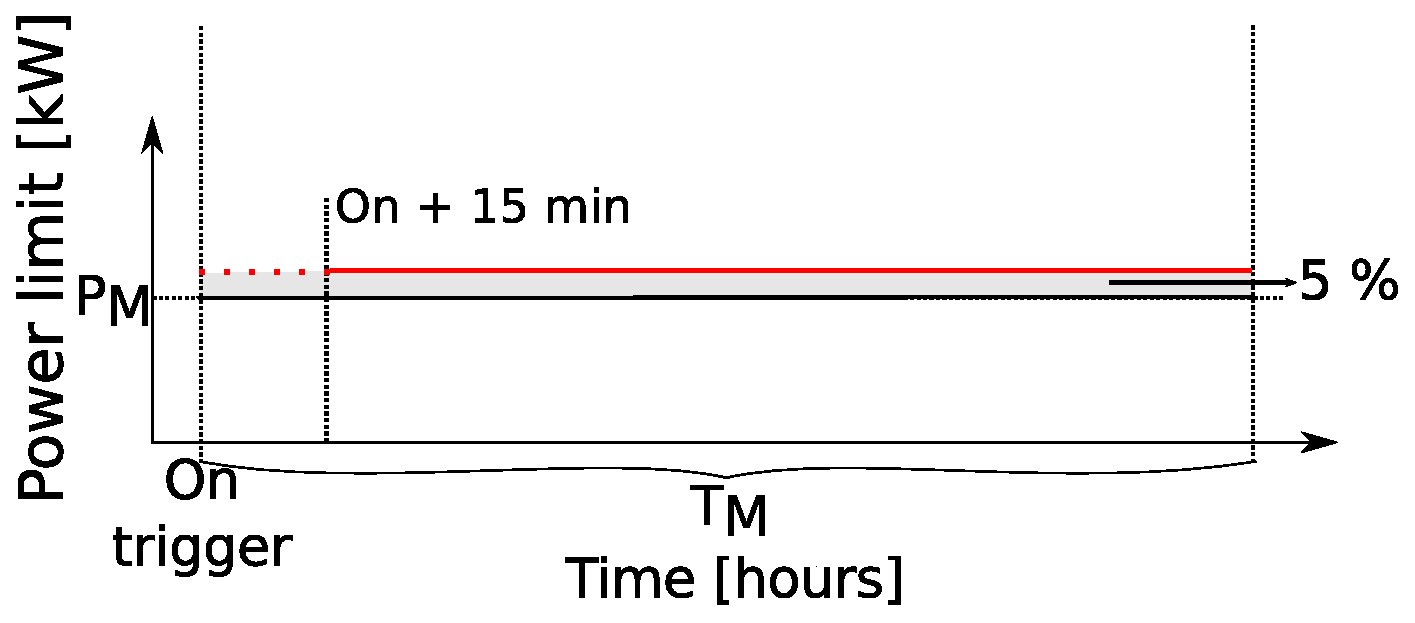
\includegraphics[width=2.5in]{isgt2014/drawing3.eps}
	\caption{The PowerMax service requirements, where the red line represents the boundaries for the permissible error, and the shaded area represents the error in service delivery, which is within the limits established in the QoS. }\label{fig:servicereq}
\end{figure}

	
% section the_performance_index (end)
